\epi{``对此感兴趣,并且希望做点什么。''}
{\textit{在为~Go 添加复数支持时}\\ \textsc{KEN THOMPSON}}

\noindent{}什么是~Go?来自其网站\cite{go_web}的介绍:
\begin{quote}
Go 编程语言是一个使得程序员更加有效率的开源项目。Go 是有表达力、简洁、清晰和有效率的。
它的并行机制使其很容易编写多核和网络应用,而新奇的类型系统允许构建有弹性的模块化程序。
Go 编译到机器码非常快速,同时具有便利的垃圾回收和强大的运行时反射。
它是快速的、静态类型编译语言,但是感觉上是动态类型的,解释型语言。
\end{quote}

Go 1 是~Go 语言的第一个稳定发布版本。
本文档的所有练习都工作于~Go 1 -- 如果不能工作,那就一定是~bug。

本书使用了下面的约定:
\begin{itemize}
\item 代码、关键字和注释使用~\prog{Source Code Pro} 显示;
\item 代码中的额外标识~\coderemark{像这样显示};
\item 较长的标识提供数字 -- \gocircle{1} -- 详细解释在其后显示;
\item (如果需要)行号在右边显示;
\item shell 的例子使用~\pr{} 作为输入符;
\item 用户在~shell 输入内容的例子~\texttt{\user{用黑体显示}},系统反馈~\texttt{用普通的黑体显示};
\item 强调的段落会缩进,并在左边有竖线。
\end{itemize}

\section{官方文档}
Go 已经有大量的文档。
\gomarginpar{在互联网上搜索时,应当使用``golang''这个词来代替原始的``go''。}
例如~Go Tutorial \cite{go_tutorial} 和~Effective Go \cite{effective_go}。
网站~\url{http://golang.org/doc/} 也是绝佳的起点 
\footnote{\url{http://golang.org/doc/} 本身是由~\prog{godoc} 提供服务的。}。
虽然并不一定要阅读这些文档,但是强烈建议这么做。

Go 1 通过叫做~\prog{godoc}
的标准程序提供其文档。如果你想了解内建相关(参阅下一章
``\titleref{sec:builtins}''小节)的文档,可以像这样获取:
\begin{display}
\pr \user{godoc builtin}
\end{display}

在第~\ref{chap:packages} 章解释了如何构造你自己的包的文档。

有一些特性让~Go 与众不同。
\begin{description}
\item[清晰并且简洁]
Go 努力保持小并且优美,你可以在短短几行代码里做许多事情;

\item[并行]
Go 让函数很容易成为\emph{非常}轻量的线程。
这些线程在~Go 中被叫做~\first{goroutines}{goroutines} 
\footnote{是的,它的发音很接近~\emph{co}routines,
但是~goroutines 确实有一些不同,我们将在第~\ref{chap:channels} 章讨论。};

\item[Channel]
这些~goroutines 之间的通讯由~\first{channel}{channel}\cite{hoare, csp} 完成;

\item[快速]
编译很快,执行也很快。目标是跟~C 一样快。编译时间用秒计算;

\item[安全]
当转换一个类型到另一个类型的时候需要显式的转换并遵循严格的规则。
Go 有垃圾收集,在~Go 中无须~\func{free()},语言会处理这一切;

\item[标准格式化]
Go 程序可以被格式化为程序员希望的(几乎)任何形式,
但是官方格式是存在的。标准也非常简单:
\prog{gofmt} 的输出就是\emph{官方认可的格式};

\item[类型后置]
类型在变量名的\emph{后面},像这样~\prog{var a int},
来代替~C 中的~\prog{int a};

\item[UTF-8]
任何地方都是~UTF-8的,包括字符串\emph{以及}程序代码。 
你可以在代码中使用~\prog{$\Phi$ = $\Phi$ + 1};

\item[开源]
Go 的许可证是完全开源的,参阅~Go 发布的源码中的~LICENSE 文件;

\item[开心]
用~Go 写程序会非常开心!

\end{description}
Erlang\cite{erlang} 与~Go 在部分功能上类似。
Erlang 和~Go 之间主要的区别是~Erlang 是函数式语言,而~Go 是命令式的。
Erlang 运行在虚拟机上,而~Go 是编译的。Go 用起来感觉更接近~Unix。

\section{Hello World}
\label{sec:hello world}
在~Go 指南中,用一个传统的方式展现了~Go:让它打印``Hello World''
(Ken Thompson 和~Dennis Ritchie 在~20 世纪~70 年代,发布~C 语言的时候开创了这个先河)。
我们不认为其他方法可以做得更好,所以就是这个吧:Go 的``Hello World''。

\lstinputlisting[numbers=right,label=src:hello,caption=Hello world]{src/helloworld.go}
逐行阅读这个程序。
\showremarks

\section{编译和运行代码}
\label{sec:building a program}
构建~Go 程序的最佳途径是使用~\prog{go} 工具。\index{tooling!go}

构建~\prog{helloworld} 只需要:
\begin{display}
\pr \user{go build helloworld.go}
\end{display}
\index{tooling!go!build}
结果是叫做~\prog{helloworld} 的可执行文件。

\begin{display}
\pr \user{./helloworld}
\end{display}

\vspace{-3.0ex}
\texttt{Hello, world; or }%
\begin{math}\kappa\alpha\lambda\eta\mu\acute{\epsilon}\rho\alpha\hspace{1em}\kappa\end{math}%
\'o\begin{math} \sigma\mu\epsilon\end{math}\texttt{; or }こんにちは 世界
\ \newline
\ \newline

\section{本书使用的设置}
\label{sec:settings_used}
\begin{itemize}                            
\item Go 被安装在~\file{\~{}/go},而~\var{\$GOROOT} 被设置为~\var{GOROOT=\~{}/go};
\item 希望编译的~Go 代码放在~\file{\~{}/g/src} 
而~\var{\$GOPATH} 设置为~\var{GOPATH=\~{}/g}。在使用包的时候需要用到这个变量(参阅第~\ref{chap:packages} 章)。
\end{itemize}

\section{变量、类型和关键字}
\label{sec:vars}
在接下来的章节中,我们将会了解这个新语言的变量、基本类型、关键字和控制流。
Go 在语法上有着类~C 的感觉。
如果你希望将两个(或更多)语句放在一行书写,它们必须用分号(';')分隔。
一般情况下,你不需要分号。

Go 同(大多数)其他语言不同的地方在于变量的类型在变量名的\emph{后面}。
不是:\lstinline{int a},而是~\lstinline{a int}。
当定义了一个变量,它默认赋值为其类型的 null 值。
这意味着,在~\lstinline{var a int}后,\lstinline{a} 的值为~0。
而~\lstinline{var s string},意味着~\lstinline{s} 被赋值为零长度字符串,
也就是~\lstinline{""}。

在~Go 中,声明和赋值是两过程,但是可以连在一起。
比较下面作用相同的代码片段。
\index{variables!declaring}
\index{variables!assigning}

\begin{minipage}{.5\textwidth}
\begin{lstlisting}[linewidth=.5\textwidth,caption={用 = 声明}]
var a int
var b bool
a = 15
b = false
\end{lstlisting}
\hfill
\end{minipage}
\begin{minipage}{.5\textwidth}
\begin{lstlisting}[linewidth=.5\textwidth,caption={用 := 声明}]
a := 15
b := false
\end{lstlisting}
\ \\
\ \\
\hfill
\end{minipage}

在左边使用了关键字~\key{var} 声明变量,\emph{然后}赋值给它。
右边的代码使用了~\mbox{\key{:=}{ }} 使得在一步内完成了声明和赋值
(这一形式只可用在函数\emph{内})。
在这种情况下,变量的类型是由值\emph{推演}出来的。
值~15 表示是~\type{int} 类型,值~\texttt{false} 告诉~Go 它的类型应当是~\type{bool}。
多个~\key{var} 声明可以成组;\key{const} 和~\key{import} 同样允许这么做。
留意圆括号的使用:
\begin{lstlisting}
var (
    x int
    b bool
)
\end{lstlisting}
有相同类型的多个变量同样可以在一行内完成声明:
\lstinline{var x, y int} 让~\var{x} 和~\var{y} 都是~\type{int} 类型变量。
同样可以使用~\first{平行赋值}{parallel assignment}:
\begin{lstlisting}
a, b := 20, 16
\end{lstlisting}
让~\var{a} 和~\var{b} 都是整数变量,并且赋值~20 给~\var{a},16 给~\var{b}。

一个特殊的变量名是~\var{\textbf{\_}}\index{variables!\_}(下划线)\index{variables!underscore}。
任何赋给它的值都被丢弃。在这个例子中,将~35 赋值给~\var{b},同时丢弃~34。
\begin{lstlisting}
_, b := 34, 35
\end{lstlisting}
Go 的编译器对声明却\emph{未使用}的变量会报错。下面的代码会产生这个错误:
\error{声明了~i 却未使用}

\begin{lstlisting}
package main
func main() { 
    var i int
}
\end{lstlisting}

\subsection{布尔类型}
布尔类型表示由预定义的常量~\emph{true} 和~\emph{false} 代表的布尔判定值。
布尔类型是~\type{bool}。

\subsection{数字类型}
Go 有众所周知的类型如~\lstinline{int},这个类型根据你的硬件决定适当的长度。
意味着在~32 位硬件上,是~32 位的;在~64 位硬件上是~64 位的。
注意:\lstinline{int} 是~32 或~64 位之一,不会定义成其他值。
\lstinline{uint} 情况相同。

如果你希望明确其长度,你可以使用~\type{int32} 或者~\type{uint32}。
完整的整数类型列表(符号和无符号)是~
\type{int8},\type{int16},\type{int32},\type{int64} 和~
\type{byte},\type{uint8},\type{uint16},\type{uint32},\type{uint64}。
\lstinline{byte} 是~\lstinline{uint8} 的别名。
浮点类型的值有~\type{float32} 和~\type{float64}
(没有~\lstinline{float} 类型)。 
64 位的整数和浮点数\emph{总是}~64 位的,即便是在~32 位的架构上。

需要留意的是这些类型全部都是独立的,并且混合用这些类型向变量赋值会引起编译器错误,
例如下面的代码:
\lstinputlisting[numbers=right,label=src:types,caption=相似的类型都是独立的]{src/types.go}
在行~7 触发一个赋值错误:

\noindent\error{types.go:7: cannot use a + a (type int)  as type int32 in assignment}

赋值可以用八进制、十六进制或科学计数法:
\lstinline{077},\lstinline{0xFF},\lstinline{1e3} 或者~
\mbox{\lstinline{6.022e23}} 这些都是合法的。

\subsection{常量}
\label{sec:constants}
常量在~Go 中,也就是~constant。它们在编译时被创建,只能是数字、字符串或布尔值;
\lstinline{const x = 42} 生成~\var{x} 这个常量。可以使用~\first{\key{iota}}{keyword!iota}
\footnote{单词~[iota] 在日常英语短语``not one iota'',意思是``不是最小'',
是来自新约中的短语:``\emph{until heaven and earth pass away, not an
iota, not a dot, will pass from the Law}.''\cite{iota}}
生成枚举值。
\begin{lstlisting}
const (
	a = iota
	b = iota 
)
\end{lstlisting}
第一个~\key{iota} 表示为~0,因此~\var{a} 等于~0,
当~\key{iota} 再次在新的一行使用时,它的值增加了~1,
因此~\var{b} 的值是~1。

也可以像下面这样,省略~Go 重复的~\key{= iota}:
\begin{lstlisting}
const (
	a = iota
	b	    |\coderemark{Implicitly \texttt{b = iota}}|
)
\end{lstlisting}
如果需要,可以明确指定常量的类型:
\begin{lstlisting}
const (
	a = 0           |\coderemark{Is an \key{int} now}|
	b string = "0" 
)
\end{lstlisting}

\subsection{字符串}
另一个重要的内建类型是~\lstinline{string}。赋值字符串的例子:
\begin{lstlisting}
s := "Hello World!"
\end{lstlisting}
字符串在~Go 中是~UTF-8 的由双引号(")包裹的字符序列。
如果你使用单引号(')则表示一个字符(UTF-8编码)
——这种在~Go 中\emph{不是}~\lstinline{string}。

一旦给变量赋值,字符串就不能修改了:在~Go 中字符串是不可变的。
从~C 来的用户,下面的情况在~Go 中是非法的:
\begin{lstlisting}
var s string = "hello"
s[0] = 'c'  |\coderemark{修改第一个字符为 'c',这会报错}|
\end{lstlisting}
在~Go 中实现这个,需要下面的方法:
\begin{lstlisting}
s := "hello"
c := []rune(s)	    |\longremark{转换 \var{s} 为 rune 数组,%
查阅在第 \ref{chap:beyond} 章``\titleref{sec:conversions}''节、%
\pageref{sec:conversions} 页的内容;}|
c[0] = 'c'	    |\longremark{修改数组的第一个元素;}|
s2 := string(c)     |\longremark{创建\emph{新的}字符串 \var{s2} 保存修改;}|
fmt.Printf("%s\n", s2) |\longremark{用 \func{fmt.Printf} 函数输出字符串。}|
\end{lstlisting}
\showremarks

\begin{lbar}[多行字符串]
基于分号的置入(查阅文档~\cite{effective_go}的``分号''章节),
你需要小心使用多行字符串。如果这样写:
\begin{lstlisting}
s := "Starting part"
    + "Ending part"
\end{lstlisting}
会被转换为:
\begin{lstlisting}
s := "Starting part";
    + "Ending part";
\end{lstlisting}
这是错误的语法,应当这样写:
\begin{lstlisting}
s := "Starting part" +
     "Ending part"
\end{lstlisting}
Go 就不会在错误的地方插入分号。另一种方式是使用反引号~\key{`} 作为\emph{原始}字符串符号\index{string literal!raw}:
\begin{lstlisting}
s := `Starting part
     Ending part`
\end{lstlisting}
留意最后一个例子~\var{s} 现在也包含换行。
不像\emph{转义}字符串标识~\index{string literal!interpreted} ,
原始字符串标识的值在引号内的字符是\emph{不转义}的。
\end{lbar}

\subsection{rune}
\lstinline{Rune} 是~\type{int32} 的别名。用 UTF-8 进行编码。这个类型在什么时候使用呢?例如需要遍历字符串中的字符。可以循环每个字节(仅在使用 US ASCII 编码字符串时与字符等价,而它们在 Go 中\emph{不}存在!)。因此为了获得实际的字符,需要使用 \type{rune} 类型。

\subsection{复数}
Go 原生支持复数。它的变量类型是~\lstinline{complex128}
(64 位虚数部分)。如果需要小一些的,还有~\lstinline{complex64}~-- 
32 位的虚数部分。复数写为~\var{re + im$i$},\var{re} 是实数部分,
\var{im} 是虚数部分,而~$i$ 是标记~'$i$' ($\sqrt{-1}$)。
使用复数的一个例子:

\gomarginpar{Printf() 的 \%v 参数含义是``用默认格式打印这个值''。}
\lstinline{var c complex64 = 5+5i; fmt.Printf("Value is: %v", c)}\newline
将会打印:\lstinline{(5+5i)}

\subsection{错误}
任何足够大的程序或多或少都会需要使用到错误报告。因此~Go 有为了错误而存在的内建类型,叫做~\lstinline{error}。

\lstinline{var e error} 定义了一个 \lstinline{error} 类型的变量 \var{e},其的值是 \lstinline{nil}。
这个 error 类型是一个接口——在第``\titleref{chap:interfaces}''章将会对此进行解释。

\section{运算符和内建函数}
\label{sec:builtins}
Go 支持普通的数字运算符,表格~\ref{tab:op-precedence} 列出了当前支持的运算符,
以及其优先级。它们全部是从左到右结合的。

\begin{table}[H]
\begin{center}
\caption{运算优先级}
\label{tab:op-precedence}
\begin{tabular}{ll}
\textbf{precedence} & \textbf{operator(s)} \\ \hline
highest   &	\verb!*  /  %  <<  >>  &  &^!		\\
    &	\verb!+  -  | ^!			\\
    &	\verb+==  !=  <  <=  >  >=+		\\
    &	\verb!<-!				\\
    &	\verb!&&!				\\
lowest    &	\verb!||!				\\
\end{tabular}

\end{center}
\end{table}
\verb|+ - * /| 和~\verb|%| 会像你期望的那样工作,
\verb!& | ^! 和~\verb!&^! 分别表示位运算符\first{按位与}{operator!bitwise!and},
\first{按位或}{operator!bitwise!or},\first{按位异或}{operator!bit
wise xor}和\first{位清除}{operator!bitwise!clear}。
\verb|&&| 和~\verb/||/ 运算符是逻辑\first{与}{operator!and}和逻辑
\first{或}{operator!or}。表格中没有列出的是逻辑\first{非}{operator!not}:\verb/!/。

虽然~Go 不支持运算符重载(或者方法重载),而一些内建运算符却\emph{支持}重载。
例如~\texttt{+} 可以用于整数、浮点数、复数和字符串(字符串相加表示串联它们)。

\section{Go 关键字}
\begin{table}[H]
\begin{center}
\caption{Go 中的关键字}
\label{tab:keywords}
%%%%%%%%%%%%%%%%%%%%%%%%%%%%%%%%%%%%%%%%%%%%%%%%%%%%%%%%%%%%%%%%%%%%%%
%%                                                                  %%
%%  This is a LaTeX2e table fragment exported from Gnumeric.        %%
%%                                                                  %%
%%%%%%%%%%%%%%%%%%%%%%%%%%%%%%%%%%%%%%%%%%%%%%%%%%%%%%%%%%%%%%%%%%%%%%
\begin{tabular}{lllll}
\key{break}	&\key{default}          &\key{for}	&\key{import}    &\key{return}\\
\key{case}	&\key{defer}            &\key{func}	&\key{interface}          &\key{select}\\
\key{chan}	&\key{delete}           &\key{go}	&\key{map}      &\key{struct}\\
\key{const}	&\key{else}    	    &\key{goto}	&\key{package}        &\key{switch}\\
\key{continue}	&\key{fallthrough}      &\key{if}	&\key{range}       &\key{type}\\
               &                       &               &                   &\key{var}\\
\end{tabular}

\end{center}
\end{table}
表格~\ref{tab:keywords} 列出了~Go 中所有的关键字。
在下面的段落和章节中会介绍它们。其中有一些已经遇到过了。
\begin{itemize}
\item \key{var} 和~\key{const} 参阅``\titleref{sec:vars}''在第~\pageref{sec:vars} 页;
\item 在``\titleref{sec:hello world}''部分,\key{package} 和~\key{import} 已经有过短暂的接触。 
在第~\ref{chap:packages} 章对其有详细的描述。
\end{itemize}
其他都有对应的介绍和章节:
\begin{itemize}
\item \key{func} 用于定义函数和方法;
\item \key{return} 用于从函数返回,\key{func} 和~\key{return}
参阅第~\ref{chap:functions} 章了解详细信息;
\item \key{go} 用于并行,参阅第~\ref{chap:channels} 章;
\item \key{select} 用于选择不同类型的通讯,参阅第~\ref{chap:channels} 章;
\item \key{interface} 参阅第~\ref{chap:interfaces} 章;
\item \key{struct} 用于抽象数据类型,参阅第~\ref{chap:beyond} 章;
\item \key{type} 同样参阅第~\ref{chap:beyond} 章。
\end{itemize}

\section{控制结构}
在~Go 中只有很少的几个控制结构
\footnote{这个章节复制于~\cite{effective_go}。}。
例如这里没有~do 或者~while 循环,只有~\key{for}。
有(灵活的)\key{switch} 语句和~\key{if},而
\key{switch} 接受像~\key{for} 那样可选的初始化语句。
还有叫做类型选择和多路通讯转接器的~\key{select}(参阅第~\ref{chap:channels} 章)。
语法有所不同(同~C 相比):无需圆括号,而语句体必须\emph{总是}包含在大括号内。

\subsection{if-else}
在~Go 中~\first{\key{if}}{keyword!if} 看起来是这样的:
\begin{lstlisting}
if x > 0 {	|\coderemark{\{ 是强制的}|
    return y
} else {
    return x
}
\end{lstlisting}
强制大括号鼓励将简单的~\key{if} 语句写在多行上。
无论如何,这都是一个很好的形式,尤其是语句体中含有控制语句,
例如~\first{\key{return}}{keyword!return} 或者~\first{\key{break}}{keyword!break}。

\key{if} 和~\key{switch} 接受初始化语句,通常用于设置一个(局部)变量。
\begin{lstlisting}
if err := Chmod(0664); err != nil { |\coderemark{\texttt{nil} 与 C 的 NULL 类似}|
    fmt.Printf(err) |\coderemark{\var{err} 的作用域被限定在 \key{if} 内}|
    return err
}
\end{lstlisting}
可以像通常那样使用逻辑运算符(参考~\ref{tab:op-precedence} 表格):
\begin{lstlisting}
if true && true  {
    fmt.Println("true")
}
if ! false {
    fmt.Println("true")
}
\end{lstlisting}

在~Go 库中,你会发现当一个~\key{if} 语句不会进入下一个语句流程~-- 
也就是说,语句体结束于~\key{break},\key{continue},\key{goto}
或者~\key{return}~-- 不必要的~\first{\key{else}}{keyword!else} 会被省略。

\begin{lstlisting}
f, err := os.Open(name, os.O_RDONLY, 0)
if err != nil {
    return err
}
doSomething(f)
\end{lstlisting}
这个例子通常用于检测可能的错误序列。成功的流程一直执行到底部使代码很好读,
当遇到错误的时候就排除它。这样错误的情况结束于~\key{return} 语句,
这样就无须~\key{else} 语句。
\begin{lstlisting}
f, err := os.Open(name, os.O_RDONLY, 0)
if err != nil {
    return err
}
d, err := f.Stat()
if err != nil {
    return err
}
doSomething(f, d)
\end{lstlisting}
下面的语法在~Go 中是非法的:
\begin{lstlisting}
if err != nil
{		    |\coderemark{必须同~if 在同一行}|
    return err
}
\end{lstlisting}
参阅文档\cite{effective_go}的``分号''章节了解其后更深入的原因。


\subsection{goto}
Go 有~\first{\key{goto}}{keyword!goto} 语句——明智的使用它。
用~\key{goto} 跳转到一定是当前函数内定义的标签\index{label}。
例如假设这样一个循环:
\begin{lstlisting}
func myfunc() {
        i := 0                                                                                      
Here:	   |\coderemark{这行的第一个词,以冒号结束作为标签}|
        println(i)
        i++ 
        goto Here |\coderemark{跳转}|
}
\end{lstlisting}
标签名是大小写敏感的。

\subsection{for}
\label{sec:for}
Go 的~\first{\key{for}}{keyword!for} 循环有三种形式,只有其中的一种使用分号。
\begin{lstlisting}
for init; condition; post { } |\coderemark{和~C 的~\key{for} 一样}|

for condition { }             |\coderemark{和~while 一样}|

for { }                       |\coderemark{死循环}|
\end{lstlisting}
短声明使得在循环中声明一个序号变量更加容易。
\begin{lstlisting}
sum := 0
for i := 0; i < 10; i++ {
    sum += i	|\coderemark{sum = sum + i 的简化写法}|
}   |\coderemark{\var{i} 实例在循环\emph{结束}会消失}|
\end{lstlisting}
最后,由于~Go 没有逗号表达式,而~++ 和~-- 是语句而不是表达式,
如果你想在~\key{for} 中执行多个变量,应当使用~\first{平行赋值}{parallel assignment}。
\begin{lstlisting}
// Reverse a
for i, j := 0, len(a)-1; i < j; i, j = i+1, j-1 {
    a[i], a[j] = a[j], a[i] |\coderemark{平行赋值}|
}
\end{lstlisting}

\subsection{break 和~continue}
利用~\first{\key{break}}{keyword!break} 可以提前退出循环,\key{break} 终止当前的循环。
\begin{lstlisting}
for i := 0; i < 10; i++ {
    if i > 5 {
	break |\coderemark{终止这个循环,只打印~0 到~5}|
    }
    println(i)
}
\end{lstlisting}
循环嵌套循环时,可以在~\key{break} 后指定标签。
用标签决定\emph{哪个}循环被终止:
\begin{lstlisting}
J:  for j := 0; j < 5; j++ {
	for i := 0; i < 10; i++ {
	    if i > 5 { 
		break J	|\coderemark{现在终止的是 \var{j} 循环,而不是 \var{i} 的那个}|
	    }
	    println(i)
	}
    } 
\end{lstlisting}

利用~\first{\key{continue}}{keyword!continue} 让循环进入下一个迭代,而略过剩下的所有代码。
下面循环打印了~0 到~5。
\begin{lstlisting}
for i := 0; i < 10; i++ {
    if i > 5 {
	continue |\coderemark{跳过循环中所有的代码}
    println(i)
}
\end{lstlisting}

\subsection{range}
关键字~\first{\key{range}}{keyword!range} 可用于循环。
它可以在~slice、array、string、map 和~channel(参阅第~\ref{chap:channels} 章)。
\key{range} 是个迭代器,当被调用的时候,从它循环的内容中返回一个键值对。
基于不同的内容,\key{range} 返回不同的东西。

当对~slice 或者~array 做循环时,\key{range} 返回序号作为键,这个序号对应的内容作为值。
考虑这个代码:\index{keyword!range!on slices}
\begin{lstlisting}
list := []string{"a", "b", "c", "d", "e", "f"}     |\longremark{创建一个字符串的 %
slice(参阅``\titleref{sec:arrays}''的第~\pageref{sec:arrays} 页)。}|
for k, v := range list {	|\longremark{用~\key{range} 对其进行循环。%
每一个迭代,\key{range} 将返回~\type{int} 类型的序号,%
\type{string} 类型的值,以~0 和``a''开始。}|
\longremark{\var{k} 的值为~0\ldots5,而~%
\var{v} 会循环``a''\ldots``f''。}| // 对~k 和~v 做想做的事情
}
\end{lstlisting}
\showremarks

也可以在字符串上直接使用~\key{range}。
这样字符串被打散成独立的~Unicode 字符
\footnote{在~UTF-8 世界的字符有时被称作~\first{runes}{runes}。
通常,当人们讨论字符时,多数是指~8 位字符。
UTF-8 字符可能会有~32 位,称作~rune。在这个例子里,\var{char} 的类型是 \type{rune}。}并且起始位按照~UTF-8 解析。
循环:\index{keyword!range!on maps}
\begin{lstlisting}
for pos, char := range "a|$\Phi{}$|x" {
    fmt.Printf("character '%c' starts at byte position %d\n", char, pos)
}
\end{lstlisting}
打印
\begin{display}
character 'a' starts at byte position 0
character '\begin{math}\Phi\end{math}' starts at byte position 1
character 'x' starts at byte position 3 \coderemark{\begin{math}\Phi\end{math} took 2 bytes}
\end{display}

\subsection{switch}
Go 的~\first{\key{switch}}{keyword!switch} 非常灵活。
表达式不必是常量或整数,执行的过程从上至下,直到找到匹配项,
而如果~\key{switch} 没有表达式,它会匹配~\type{true} 。
这产生一种可能——使用~\key{switch} 编写~\key{if-else-if-else} 判断序列。
\begin{lstlisting}
func unhex(c byte) byte {
    switch {
    case '0' <= c && c <= '9':
        return c - '0'
    case 'a' <= c && c <= 'f':
        return c - 'a' + 10
    case 'A' <= c && c <= 'F':
        return c - 'A' + 10
    }
    return 0
}
\end{lstlisting}
它匹配成功后不会自动向下尝试,但是可以使用
\first{\key{fallthrough}}{keyword!fallthrough}
使其这样做。
没有~\key{fallthrough}:
\begin{lstlisting}
switch i {
    case 0:  |\coderemark{空的 case 体}|
    case 1:
	f()  |\coderemark{当 i == 0 时,f 不会被调用!}|
}
\end{lstlisting}
而这样:
\begin{lstlisting}
switch i {
    case 0:  fallthrough
    case 1:
	f()  |\coderemark{当 i == 0 时,f 会被调用!}|
}
\end{lstlisting}
用~\first{\key{default}}{keyword!default} 可以指定当其他所有分支都不匹配的时候的行为。
\begin{lstlisting}
switch i {
    case 0:  
    case 1:
	f()
    default:	
        g()	|\coderemark{当 i 不等于 0 或 1 时调用}|
}
\end{lstlisting}
分支可以使用逗号分隔的列表。
\begin{lstlisting}
func shouldEscape(c byte) bool {
    switch c {
    case ' ', '?', '&', '=', '#', '+': |\coderemark{, as "or"}|
        return true
    }
    return false
}
\end{lstlisting}
这里有一个使用两个~\key{switch} 对字节数组进行比较的例子:
\begin{lstlisting}
|\longremark{比较返回两个字节数组字典数序先后的整数。
如果 a == b 返回 0,如果 a < b 返回 -1,而如果 a > b 返回 +1;}|
func Compare(a, b []byte) int {
    for i := 0; i < len(a) && i < len(b); i++ {
        switch {
        case a[i] > b[i]:
            return 1
        case a[i] < b[i]:
            return -1
        }
    }
    switch { |\longremark{长度不同,则不相等;}|
    case len(a) < len(b):
        return -1
    case len(a) > len(b):
        return 1
    }
    return 0	|\longremark{字符串相等。}|
}
\end{lstlisting}
\showremarks

\section{内建函数}
预定义了少数函数,这意味着\emph{无需}引用任何包就可以使用它们。
表格~\ref{tab:predef-functions} 列出了所有的内建函数。\footnote{可以使用命令~
\prog{godoc builtin} 获得关于内建类型和函数的在线文档。}

\begin{table}[H]
\begin{center}
\caption{Go 中的预定义函数}
\label{tab:predef-functions}
\begin{tabular}{lllll}
\key{close}	&\key{new}	&\key{panic}	&\key{complex} \\
\key{delete}   &\key{make}     &\key{recover}  &\key{real} \\
\key{len}	&\key{append}	&\key{print}	&\key{imag}  \\
\key{cap}	&\key{copy}	&\key{println}	&\\
\end{tabular}

\end{center}
\end{table}

这些内建函数的文档记录在跟随最近的 Go 版本一起发布的伪包~\package{builtin} \index{package!builtin} 中。

\begin{description}
\item[\func{close}] 用于~channel
通讯。使用它来关闭~channel,参阅第~\ref{chap:channels} 章了解更多。
\index{built-in!close}

\item[\func{delete}] 用于在~map 中删除实例。
\index{built-in!delete}

\item[\func{len} 和~\func{cap}] 可用于不同的类型,
\func{len} 用于返回字符串、slice 和数组的长度。
参阅``\titleref{sec:arrays}''小节了解更多关于~slice、
数组和函数~\func{cap} 的详细信息。
\index{built-in!len}\index{built-in!cap}

\item[\func{new}] 用于各种类型的内存分配。
参阅``\titleref{sec:allocation with new}''的第~\pageref{sec:allocation with new} 页。
\index{built-in!new}

\item[\func{make}] 用于内建类型(map、slice 和~channel)的内存分配。
参阅``\titleref{sec:allocation with make}''的第~\pageref{sec:allocation with make} 页。
\index{built-in!make}

\item[\func{copy}] 用于复制~slice。
参阅本章的``\titleref{sec:slices}''。
\index{built-in!copy}

\item[\func{append}] 用于追加~slice。
参阅本章的``\titleref{sec:slices}''。
\index{built-in!append}

\item[\func{panic}、\func{recover}] 用于\emph{异常}处理机制。
参阅``\titleref{sec:panic}''的第~\pageref{sec:panic} 页了解更多信息。
\index{built-in!panic}
\index{built-in!recover}

\item[\func{print}、\func{println}] 是底层打印函数,可以在不引入~
\package{fmt}\index{package!fmt} 包的情况下使用。它们主要用于调试。
\index{built-in!print}\index{built-in!println}

\item[\func{complex}、\func{real}、\func{imag}] 全部用于处理
\first{复数}{complex numbers}。有了之前给的简单的例子,不用再进一步讨论复数了。
\index{built-in!complex}
\index{built-in!real}
\index{built-in!imag}
\end{description}

\section{array、slices 和~map}
\label{sec:arrays}
可以利用~array 在列表中进行多个值的排序,或者使用更加灵活的:slice。
字典或哈希类型同样可以使用,在~Go 中叫做~\type{map}。

\subsection{array}
array 由~\verb|[n]<type>| 定义,$n$ 标示~array 的长度,
而~\verb|<type>| 标示希望存储的内容的类型。
对~array 的元素赋值或索引是由方括号完成的:
\begin{lstlisting}
var arr [10]int
arr[0] = 42
arr[1] = 13
fmt.Printf("The first element is %d\n", arr[0])
\end{lstlisting}
像~\lstinline{var arr = [10]int} 这样的数组类型有固定的大小。
大小是类型的\emph{一部分}。由于不同的大小是不同的类型,因此不能改变大小。
数组同样是值类型的:将一个数组赋值给另一个数组,会\emph{复制}所有的元素。
尤其是当向函数内传递一个数组的时候,它会获得一个数组的副本,而不是数组的指针。

\index{array!multidimensional}
可以像这样声明一个数组:\lstinline{var a [3]int},
如果不使用零来初始化它,则用\first{复合声明}{literal!composite}:\lstinline|a := [3]int{1, 2, 3}| 也可以简写为
\lstinline|a := [...]int{1, 2, 3}|,Go 会自动统计元素的个数。

\gomarginpar{复合声明允许你直接将值赋值给~array、slice 或者~map。

参阅第~\pageref{sec:constructors and composite literals} 页的``\titleref{sec:constructors and composite literals}''了解更多信息。}
声明一个~array 时,对于复合文法你\emph{必须}在方括号内输入些内容,数字或者三个点
(\verb|...|)。

当使用嵌套数组时可以使用下面的语法:
\begin{lstlisting}
a := [3][2]int{ {1,2}, {3,4}, {5,6} }
\end{lstlisting}

\subsection{slice}
\label{sec:slices}
slice 与~array 接近,但是在新的元素加入的时候可以增加长度。
slice 总是指向底层的一个~array。slice 是一个\emph{指向}~array 的指针,
这是其与~array 不同的地方;
slice 是\first{引用类型}{reference types},
\gomarginpar{引用类型使用~\lstinline{make} 创建。}
这意味着当赋值某个~slice 到另外一个变量,两个引用会指向同一个~array。
例如,如果一个函数需要一个~slice 参数,在其内对~slice 元素的修改也会体现在函数调用者中,
这和传递底层的~array 指针类似。
通过:
\begin{lstlisting}
sl := make([]int, 10)
\end{lstlisting}
创建了一个保存有~10 个元素的~slice。需要注意的是底层的~array 并无不同。
slice 总是与一个固定长度的~array 成对出现。其影响~slice 
的\first{容量}{slice!capacity}和\first{长度}{slice!length}。
\index{array!length}\index{array!capacity}
图~\ref{fig:array-vs-slice} 描述了下面的~Go 代码。
首先创建了~$m$ 个元素长度的 array,元素类型~\lstinline{int}:
\lstinline{var array[m]int}\newline
然后对这个~array 创建~slice:
\lstinline{slice := array[:n]}\newline
然后现在有:
\begin{itemize}
    \item[\lstinline{len(slice) == n}{} ;]
    \item[\lstinline{cap(slice) == m}{} ;]
    \item[\lstinline{len(array) == cap(array) == m}{} .]
\end{itemize}
\begin{figure}[H]
\caption{array 与 slice 对比}
\label{fig:array-vs-slice}
\begin{center}
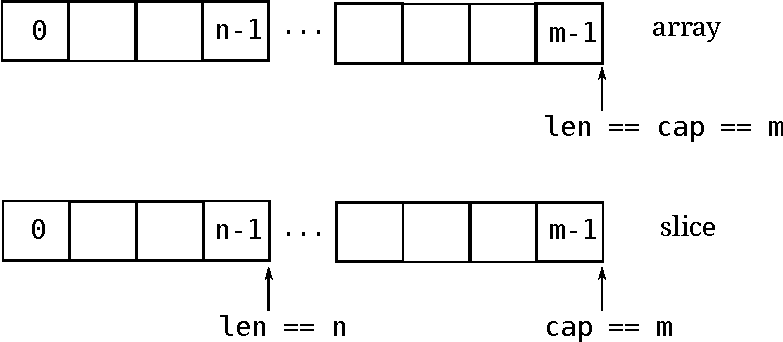
\includegraphics[scale=0.65]{fig/array-vs-slice.pdf}
\end{center}
\end{figure}

给定一个~array 或者其他~slice,一个新~slice 通过~\lstinline{a[I:J]}
的方式创建。
这会创建一个新的~slice,指向变量~\lstinline{a},从序号~\var{I} 开始,结束在序号~\var{J}之前。
长度为~\lstinline{J - I}。

\begin{lstlisting}
// array[n:m] 从~array 创建了一个~slice,具有元素~n 到~m-1
a := [...]int{1, 2, 3, 4, 5} |\longremark{定义一个~5 个元素的~array,序号从~0 到~4;}|
s1 := a[2:4] |\longremark{从序号~2 至~3 创建~slice,它包含元素~\texttt{3, 4};}|
s2 := a[1:5] |\longremark{从序号~1 至~4 创建,它包含元素~\texttt{2, 3, 4, 5};}|
s3 := a[:]   |\longremark{用~array 中的所有元素创建~slice,这是~\texttt{a[0:len(a)]} 的简化写法;}|
s4 := a[:4]  |\longremark{从序号~0 至~3 创建,这是~\texttt{a[0:4]} 的简化写法,得到~\texttt{1, 2, 3, 4};}|
s5 := s2[:]  |\longremark{从~slice \var{s2} 创建~slice,注意~\texttt{s5} 仍然指向~array \texttt{a}。}|
s6 := a[2:4:5]  |\longremark{从序号 3 到 5 创建一个 slice,\emph{并且}将容量设置为 4。}|
\end{lstlisting}
\showremarks

在~\ref{src:arrays} 列出的代码中,我们在第八行尝试做一些错误的事情,
让一些东西超出范围(底层~array 的最大长度),然后得到了一个\emph{运行时}错误。
\lstinputlisting[numbers=right,label=src:arrays,caption=array 和 slice]{src/array-and-slices.go}
如果你想要扩展~slice,有一堆内建函数让你的日子更加好过一些:
\lstinline{append} 和~\lstinline{copy}。来自于~\cite{go_spec}:
\begin{quote}
函数~\lstinline{append} 向~slice \lstinline{s} 追加零值或其他~\lstinline{x} 值,
并且返回追加后的新的、与~\lstinline{s} 有相同类型的~slice。
如果~\lstinline{s} 没有足够的容量存储追加的值,\lstinline{append} 分配一个足够大的、新的~slice
来存放原有~slice 的元素和追加的值。因此,返回的~slice 可能指向不同的底层~array。
\end{quote}
\index{built-in!append}
\begin{lstlisting}
s0 := []int{0, 0}
s1 := append(s0, 2)|\longremark{追加一个元素,\texttt{s1 == []int\{0, 0, 2\}};}|
s2 := append(s1, 3, 5, 7)|\longremark{追加多个元素,\texttt{s2 == []int\{0, 0, 2, 3, 5, 7\}};}|
s3 := append(s2, s0...)|\longremark{追加一个 slice,\texttt{s3 == []int\{0, 0, 2, 3, 5, 7, 0, 0\}}。注意这三个点!}|
\end{lstlisting}
\showremarks
还有
\begin{quote}
函数~\lstinline{copy} 从源~slice \lstinline{src} 复制元素到目标~\lstinline{dst},
并且返回复制的元素的个数。源和目标可能重叠。元素复制的数量是~\lstinline{len(src)} 
和~\mbox{\lstinline{len(dst)}} 中的最小值。
\end{quote}
\index{built-in!copy}
\begin{lstlisting}
var a = [...]int{0, 1, 2, 3, 4, 5, 6, 7}
var s = make([]int, 6)
n1 := copy(s, a[0:])|\coderemark{\texttt{n1 == 6, s == []int\{0, 1, 2, 3, 4, 5\}}}|
n2 := copy(s, s[2:])|\coderemark{\texttt{n2 == 4, s == []int\{2, 3, 4, 5, 4, 5\}}}|
\end{lstlisting}

\subsection{map}
\label{sec:maps}
许多语言都内建了类似的类型,例如~Perl 有哈希,Python 有字典,
而~C++ 同样也有~map(作为库)。 
在~Go 中有 \first{\key{map}}{keyword!map} 类型。\type{map} 
可以认为是一个用字符串做索引的数组(在其最简单的形式下)。
下面定义了~\type{map} 类型,用于将~\lstinline{string} (月的缩写)转换为~\lstinline{int}~-- 那个月的天数。 
一般定义~map 的方法是:\verb|map[<from type>]<to type>|

\begin{lstlisting}
monthdays := map[string]int{
	"Jan": 31, "Feb": 28, "Mar": 31, 
	"Apr": 30, "May": 31, "Jun": 30, 
	"Jul": 31, "Aug": 31, "Sep": 30, 
	"Oct": 31, "Nov": 30, "Dec": 31,|\coderemark{逗号是必须的}|
}
\end{lstlisting}
留意,当只需要声明一个~\lstinline{map} 的时候,使用~\lstinline{make} 的形式:
\lstinline|monthdays := make(map[string]int)|

当在~map 中索引(搜索)时,使用方括号。例如打印出~12 月的天数:
\lstinline{fmt.Printf("%d\n", monthdays["Dec"])}\newline
当对~array、slice、string 或者~map 循环遍历的时候,\first{\key{range}}{keyword!range}
会帮助你,每次调用,它都会返回一个键和对应的值。\index{keyword!range!on maps}
\begin{lstlisting}
year := 0
for _, days := range monthdays {|\coderemark{键没有使用,因此用~\texttt{\_, days}}|
    year += days
}
fmt.Printf("Numbers of days in a year: %d\n", year)
\end{lstlisting}
向~\type{map} 增加元素,\index{keyword!map!add elements} 可以这样做:
\begin{lstlisting}
monthdays["Undecim"] = 30|\coderemark{添加一个月}|
monthdays["Feb"]     = 29|\coderemark{闰年时重写这个元素}|
\end{lstlisting}
检查元素是否存在\index{keyword!map!existence},可以使用下面的方式\cite{go_course_day2}:
\begin{lstlisting}
var value int
var present bool

value, present = monthdays["Jan"]|\coderemark{如果存在,\texttt{present} 则有值 \key{true}}|
                           |\coderemark{或者更接近 Go 的方式}|
v, ok := monthdays["Jan"]  |\coderemark{“逗号 ok”形式}|
\end{lstlisting}
也可以从~\type{map} 中移除元素\index{keyword!map!remove elements}:
\begin{lstlisting}
delete(monthdays, "Mar")   |\coderemark{删除 "Mar" 吧,总是下雨的月份}|
\end{lstlisting}
通常来说语句~\lstinline{delete(m, x)} 会删除~map 中由~\lstinline{m[x]} 建立的实例。

\section{练习}
\begin{Exercise}[title={For-loop},difficulty=1]
\label{ex:for-loop}
\Question \label{ex:for-loop q1} Create a simple loop with the \key{for} construct. Make it loop
10 times and print out the loop counter with the \package{fmt} package.

\Question \label{ex:for-loop q2} Put the body of the loop in a separate function.

\Question \label{ex:for-loop q3} Rewrite the loop from 1. to use \key{goto}. The
keyword \key{for} may not be used.
\end{Exercise}

\begin{Answer}

\Question There are a multitude of possibilities, 
one of the solutions could be:
\lstinputlisting[label=src:for,caption=Simple for-loop]{ex-basics/src/for.go}
Lets compile this on an Intel 386 Linux machine and look at the
output.
\vskip\baselineskip
\begin{display}
\pr 8g for.go && 8l -o for for.8
\pr ./for
0
1
.
.
.
9
\end{display}
\vskip\baselineskip

\Question Next we put the body of the 
loop - the \key{fmt.Printf} - in a separate function.
\lstinputlisting[label=src:for-func,caption=Loop calls function]{ex-basics/src/for-func.go}
The presented program should be self explanatory. Note however the
"\lstinline{j int}" instead of the more usual "\lstinline{int j}" in the
function definition.
\end{Answer}


\begin{Exercise}[title={FizzBuzz},difficulty=1]
\label{ex:fizzbuzz}
\Question \label{ex:fizzbuzz q1} Solve this problem, called
the Fizz-Buzz \cite{fizzbuzz} problem:
\begin{quote}
Write a program that prints the numbers from 1 to 100. But for multiples
of three print ``Fizz'' instead of the number and for the multiples of
five print ``Buzz''. For numbers which are multiples of both three and
five print ``FizzBuzz''.
\end{quote}
\end{Exercise}

\begin{Answer}
\Question A possible
solution to this simple problem is the following program.
\lstinputlisting[label=src:fizzbuzz,caption=Fizz-Buzz]{ex-basics/src/fizzbuzz.go}
\showremarks
\end{Answer}


\begin{Exercise}[title={Strings},difficulty=1]
\label{ex:strings}
\Question \label{ex:strings q1} Create a Go program that prints
the following (up to 100 characters):
\begin{alltt}
A
AA
AAA
AAAA
AAAAA
AAAAAA
AAAAAAA
\ldots
\end{alltt}


\Question \label{ex:strings q2} Create a program that counts
the numbers of characters/runes in this string:
\begin{alltt}
asSASA ddd dsjkdsjs dk
\end{alltt}
Make it also output the number of bytes in that string.

\Question \label{ex:string q3} Extend the program from
the previous question to replace the three runes at
position 4 with 'abc'.

\end{Exercise}

\begin{Answer}

\Question The following program is an answer to the first question.
\lstinputlisting[label=string1,caption=Strings]{ex-basics/src/string1.go}

\Question To answer this question we need some help of
the \package{string}-package. First we check the documentation
with \prog{godoc strings | less}. When we read the documentation
we notice two functions: \lstinline{func Bytes(s string) []byte} and
\lstinline{func Runes(s string) []int}. Both return values are
almost what we need, namely (\type{slices}) So we return the length of 
them. Putting this together leads to the following program.
\lstinputlisting[label=string2,caption=Runes in strings]{ex-basics/src/string2.go}
\end{Answer}


\begin{Exercise}[title={Average},difficulty=4]
\label{ex:average no func}
\Question\label{ex:average no func q1} Give the code
that calculates the average of a \type{float64} slice. In
a later exercise (Q\ref{ex:avarage} you will make it into
a function.
\end{Exercise}

\begin{Answer}
\Question The following code calculates the average.
\begin{lstlisting}
sum := 0.0 
switch len(xs) {
case 0:                 |\longremark{If the length is zero, we return 0;}|
        ave = 0
default:                |\longremark{Otherwise we calculate the average;}|
        for _, v := range xs {
                sum += v
        }
        ave = sum / float64(len(xs)) |\longremark{We have to convert the value to a %
\key{float64} to make the division work.}|
}
\end{lstlisting}
\showremarks
\end{Answer}


\cleardoublepage
\section{答案}
\shipoutAnswer
